\documentclass[titlepage,a4paper]{article}

\usepackage[utf8]{inputenc} % accented characters in input

\usepackage[spanish,activeacute]{babel}
%\usepackage[margin = 1in]{geometry}
\usepackage{a4wide}
\usepackage{bookmark}
\usepackage{fancyhdr}
\usepackage{graphicx}

\pagestyle{fancy} % Encabezado y pie de página
\fancyhf{}
\fancyhead[L]{TP1  - Grupo: 38}
\fancyhead[R]{Teoría de organización de datos - FIUBA}
\renewcommand{\headrulewidth}{0.4pt}
\fancyfoot[C]{\thepage}
\renewcommand{\footrulewidth}{0.4pt}


\begin{document}

\section{Análisis Preliminar}

\subsection{Eventos}

\subsection{Conversion}

	Este evento registra a un usuario que realiza una conversión, comprando un producto.
	
	\subsubsection{Productos más comprados}
	Lo primero que podemos mirar sobre este evento es cuáles fueron los modelos más comprados:
	
	\begin{center}
	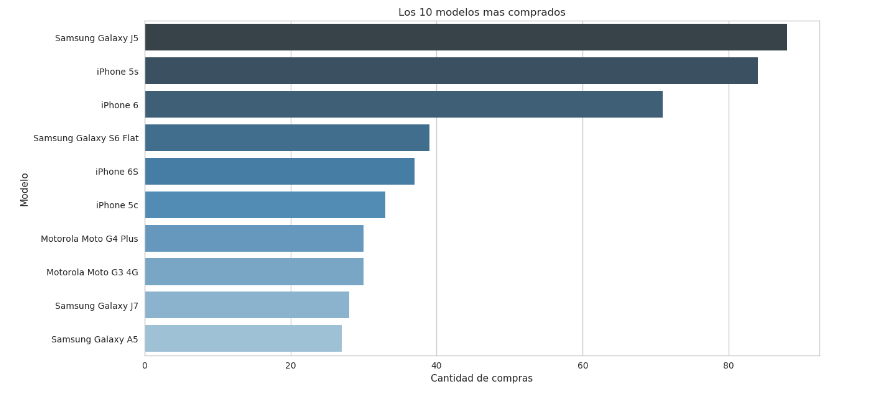
\includegraphics[width=14cm]{imagenes/top10comprados2.jpg}\\
	\textbf{Figura 2:}  \textit{En este gráfico se puede ver los 10 productos más comprados. }
	\end{center}
	
	Los tres más comprados que se pueden ver son: Samsung Galaxy J5, Iphone 5S y Iphone 6. Esos son los que más se destacan por encima del resto. Luego no hay brechas muy grandes de compras entre distintos productos. Algo que tambien es posible destacar es que, de los diez más comprados, cuatro de ellos pertenecen a la familia de los Samnsung Galaxy, cuatro son de la marca Iphone, y dos pertenecen a la familia de los Motorola Moto G.
	
	\subsubsection{Cantidad de productos comprados por condición}
	
	Gracias a la informacion provista, podemos dividir cada producto por su condicion: Nuevo, Excelente, Muy bien, Bien, Bien sin Touch ID. A partir de esto, es posible obtener cuál fue la cantidad de productos más comprados según su condición. 
	
	\begin{center}
	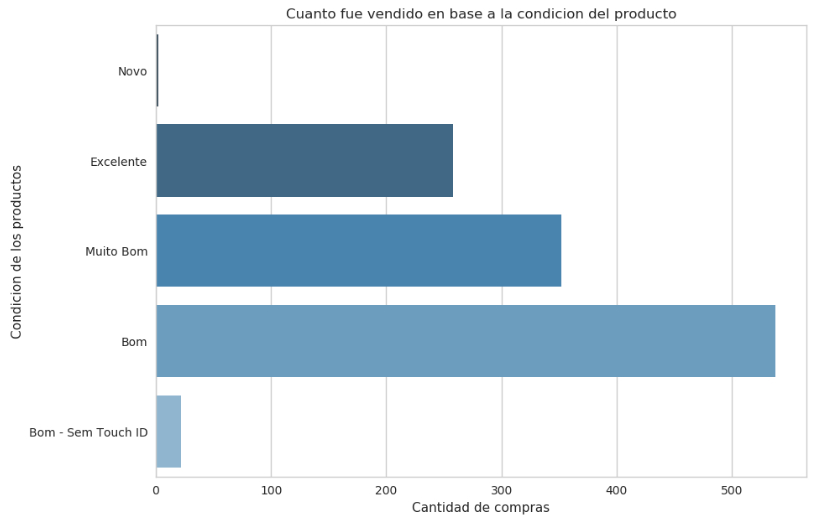
\includegraphics[width=14cm]{imagenes/compradosPorCondicion.jpg}\\
	\textbf{Figura 2:}  \textit{En este gráfico se puede ver la cantidad de procutos comprados por condicion del producto. }
	\end{center}
 
  Aquí se puede observar que los que más compras tienen son los que tienen, relativamente, peor condicion (condición: Bien). Esto puede llevar a pensar que gran parte de los usuarios al hacer una compra no priorizan la condición del producto. Aunque cabe destacar que se deberia tener en cuenta cuantos productos de cada condicion posee la pagina.
   
 \subsection{Lead}
 
 Este evento representa: El usuario se registra para recibir una notificación de disponibilidad de stock para un producto que no se encontraba disponible en ese momento.
 
  \subsubsection{Modelos con más pedidos de notificación de stock}
  
  Los viente modelos con más pedidos de notificación de stock fueron los siguientes:
  
  \begin{center}
   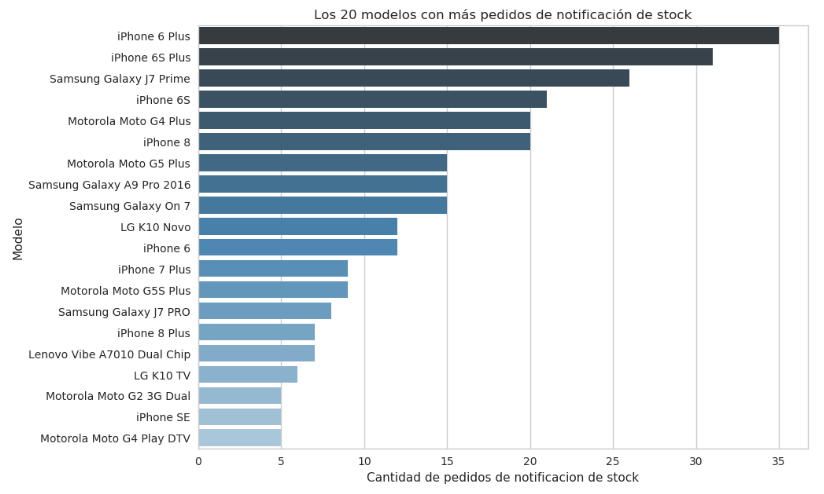
\includegraphics[width=14cm]{imagenes/top20lead.jpg}\\
	\textbf{Figura:}  \textit{Los 20 productos con más pedidos de notificación de stock.}
	\end{center}
  
 
 \subsection{Relaciones entre eventos}

  \subsubsection{Relación entre numero de compras y de visitas a productos de un usuario}
  
  Un posible análisis para esta sección es tomar cada usuario que entró alguna ves al sitio y ver cuantas compras y cuantas visitas a productos posee.
  
  Para eso se realizó un scatter plot en donde cada punto en el plano es un cliente que posee una cantidad total de visitas al sitio (eje \textit{y}) y una cantidad total de compras (eje  \textit{x}).
  
  \begin{center}
   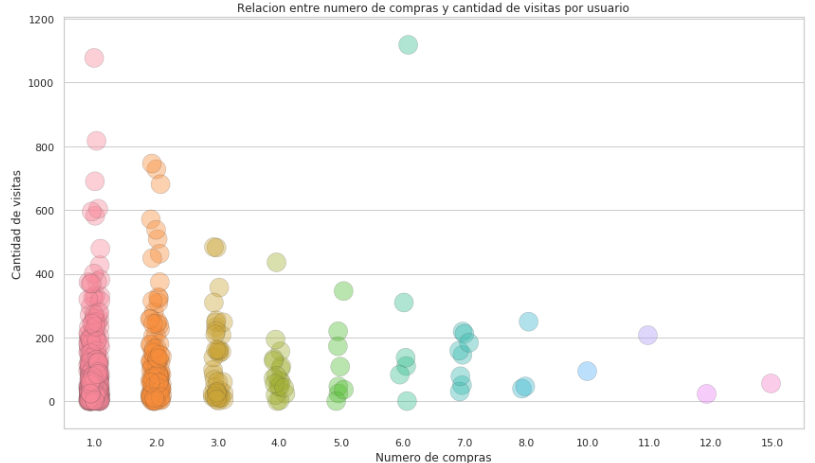
\includegraphics[width=14cm]{imagenes/comprasVsVisitas.jpg}\\
	\textbf{Figura:}  \textit{Relacion entre numero de compras y cantidad de visitas por usuario.}
	\end{center}
	
	
  \subsubsection{Relacion entre entradas al sitio por campaña y compras de productos}

  \section{Entradas de usuarios}


\end{document}